\chapter{ Chapitre 2: Architecture 
\centering logicielle et outils de travail}
\begin{spacing}{1.2}
\minitoc
\thispagestyle{MyStyle}
\end{spacing}
\newpage
\begin{sloppypar} 

\section{Introduction}
\vspace{-3mm}
Dans le chapitre précédent, nous avons abordé l’étude du projet. Dans ce nouveau chapitre, nous allons commencer par dresser la liste des acteurs qui interagissent avec le système. Ensuite, nous définirons les besoins fonctionnels et non fonctionnels de notre solution. En nous appuyant sur cette analyse, nous élaborerons une spécification détaillée de la solution choisie en utilisant des diagrammes de cas d’utilisation. Ce sprint est consacré à comprendre l’architecture logicielle et à mettre en œuvre cette dernière à travers les frameworks de développement.
\vspace{-9mm}
\section{Capture des besoins}
\vspace{-4mm}
\subsection{Définition des acteurs }
\vspace{-3mm}
Un acteur représente l’abstraction d’un rôle joué par des entités externes quiinteragissent
directement avec le système étudié. Notre application va contenir deux acteurs :

\begin{itemize}
    \item[$\bullet$] Admin : Le superviseur possède tous les droits d'accès aux paramètres de l'application web et mobile.
    \item[$\bullet$] Étudiant : Habituellement, il a accès à son compte. Il a la capacité de consulter, d'afficher, de modifier son profil et de créer des publications.
\end{itemize}
\vspace{-9mm}

\subsection{Besoins fonctionnels }
\vspace{-3mm}
Les besoins fonctionnels seront traduits par les services offerts par notre futur système.
Ils identifient les tâches ou les activités qui doivent être formulées par l’application pour les différents types d’acteurs. Pour notre futur système, les fonctionnalités sont très riches. Nous
proposons de les classer selon les acteurs responsables comme suit :
\begin{itemize}
\item [•] \textbf{Le Admin} doit être capable de :

→ S’authentifier : Saisir un login et un mot de passe pour accéder à son espace.\\
→ Gérer le profil :L'admin peut modifier ses informations personnelles.\\
→ Consulter la liste des utilisateurs de l’application.\\
→ Consulter la liste des Endroits de l’application.\\
→ Consulter la liste des evenements de l’application.\\
→ Consulter la liste des universites de l’application.\\
→ Consulter la liste des stages de l’application.\\
→ Consulter la liste des moyens de transport de l’application.\\
→ Communiquer avec les utlisateurs  de l’application.\\
→ Créer une publication sur  l’application.\\
→ Commenter sur  une publication dans  l’application.

\item [•] \textbf{L'etudiant } doit être capable de :

→ S’inscrire : L'etudiant doit créer un compte pour pouvoir accéder à l’application mobile.\\
→ S’authentifier :Saisir un login et un mot de passe pour accéder à son espace.\\
→ Gérer le profil :L'etudiant peut modifier ses informations personnelles.\\
→ communiquer avec l'admin de l’application.\\
→ créer une publication sur  l’application.\\
→ commenter sur  une publication dans  l’application.
\end{itemize}
\vspace{-5mm}
\subsection{Besoins non-fonctionnels}
\vspace{-3mm}
Les besoins non fonctionnels représentent les contraintes internes et externes à vérifier pour le futur système. Parmi les besoins non fonctionnels de notre futur système, nous pouvons citer :

\begin{itemize}
    \item Besoins d’utilisation : le système doit fournir des interfaces ergonomiques, claires et simples à utiliser.
    \item La performance : L’application à développer doit être principalement performante, c’est-à-dire, à travers ses fonctionnalités, elle doit répondre correctement à toutes les exigences des usagers.
    \item Besoins de sécurité : Le système doit interdire l’accès de tout intrus par les droits et les privilèges d’accès.
    \item L’extensibilité : La caractéristique open source de l’application va permettre son extensibilité en rajoutant de nouvelles fonctionnalités ou en modifiant des fonctionnalités déjà développées.
\end{itemize}

\vspace{-2cm}


\section{Backlog de produit  }
\vspace{-7mm}
Le backlog du produit est le cœur de Scrum. C’est ici que tout commence. Un backlog du produit est essentiellement une liste hiérarchisée d’exigences, d’histoires, de fonctionnalités ou d'autres contenus. Il représente ce que le client souhaite, décrit en termes de client. Le tableau suivant décrit le « Backlog du produit » et présente les « Histoires utilisateurs ».

\vspace{19mm}

\vspace{-2cm}
\begin{longtable}{|p{1.5cm}|p{11cm}|p{2cm}|}
\hline
\textbf{Priorité} & \textbf{Histoire Utilisateur} & \textbf{Complexité} \\
\hline
\endfirsthead
\hline
Priorité & Histoire Utilisateur & Complexité \\
\hline
\endhead
1 & En tant qu’un étudiant, je peux créer un compte dans l’application mobile. & Moyenne \\
\hline
2 & En tant qu’un utilisateur, je peux réinitialiser mon mot de passe sur la partie mobile. & Simple \\
\hline
3 & En tant qu’un utilisateur (administrateur et étudiant), je peux m’authentifier dans l’application mobile. & Moyenne \\
\hline
4 & En tant qu’un administrateur, je peux m’authentifier à l’application web. & Moyenne \\
\hline
5 & En tant qu’un administrateur, je peux supprimer les étudiants depuis l’application web. & Simple \\
\hline
6 & En tant qu’un utilisateur, je peux modifier les données de mon compte. & Difficile \\
\hline
7 & En tant qu’un étudiant, je peux gérer mon compte. & Difficile \\
\hline
8 & En tant qu’un administrateur, je peux gérer les universités dans l’application web. & Moyenne \\
\hline
9 & En tant qu’un administrateur, je peux gérer les événements dans l’application web. & Moyenne \\
\hline
10 & En tant qu’un administrateur, je peux gérer les facilités dans l’application web. & Moyenne \\
\hline
11 & En tant qu’un administrateur, je peux gérer les offres de stages dans l’application web. & Moyenne \\
\hline
12 & En tant qu’un administrateur, je peux gérer les stations de transports dans l’application web. & Moyenne \\
\hline
13 & En tant qu’un administrateur, je peux gérer les examens dans l’application web. & Moyenne \\
\hline
14 & En tant qu’un utilisateur, je peux consulter les examens sur l'application mobile. & Moyenne \\
\hline
15 & En tant qu’un étudiant, je peux consulter la carte avec filtrage des données. & Difficile \\
\hline
16 & En tant qu’un étudiant, je peux consulter les détails des facilités qui apparaissent dans la carte dans l’application mobile. & Moyenne \\
\hline
17 & En tant qu’un étudiant, je peux consulter la carte Map pour chercher les facilités et les moyens de transport. & Moyenne \\
\hline
18 & En tant qu’un étudiant, je peux consulter les localisations des événements et stages dans la carte. & Moyenne \\
\hline
19 & En tant qu’un étudiant, je peux consulter les publications de ma page d’accueil dans l’application mobile. & Moyenne \\
\hline
20 & En tant qu’un étudiant, je peux consulter mes publications de ma page profil dans l’application mobile. & Simple \\
\hline
21 & En tant qu’un étudiant, je peux commenter et réagir aux publications dans l’application mobile. & Difficile \\
\hline
22 & En tant qu’un étudiant, je peux supprimer mes publications dans l’application mobile. & Simple \\
\hline
23 & En tant qu’un administrateur, je peux créer des notifications personnalisées sur la partie web. & Simple \\
\hline
24 & En tant qu’un utilisateur, je peux consulter ma page profil sur la partie mobile. & Simple \\
\hline
25 & En tant qu’un étudiant, je peux contacter l’administrateur. & Simple \\
\hline
26 & En tant qu’un étudiant, je peux contacter l’administrateur sur l'application mobile. & Moyenne \\
\hline
27 & En tant qu’un administrateur, je peux consulter le tableau de bord dans l’application web. & Moyenne \\
\hline
\caption{Backlog de produit}
\end{longtable}

\vspace{-1.8cm}
\section{Découpage en sprint  }
\vspace{-5mm}
La planification de release en Scrum organise le travail en sprints pour une livraison incrémentale des fonctionnalités du produit, alignant ainsi les attentes des parties prenantes et assurant que le produit répond aux besoins du client à chaque itération. Le tableau ci-dessous détaille ce plan, incluant les "Histoires utilisateurs" pour chaque sprint ainsi que les dates de début et de fin prévues pour chaque période.\\
\\

\vspace{-2cm}
\small
\begin{center}
\begin{longtable}{|>{\raggedright}p{2.8cm}|>{\raggedright}p{8cm}|>{\raggedright\arraybackslash\small}p{1.9cm}|>{\raggedright\arraybackslash\small}p{1.8cm}|}

\hline
\textbf{Sprint} & \textbf{Tâches} & 
\textbf{Date Début} & \textbf{Date Fin} \\
\hline

\endfirsthead
\hline
Sprint & Tâches & Date Début & Date Fin \\
\hline
\endhead
Sprint 1: Gestion des Utilisateurs & 
\begin{itemize}
    \vspace{-0.8cm}
    \setlength{\leftskip}{-0.4cm}
    \item En tant qu’un étudiant, je peux créer un compte dans l’application mobile.
    \vspace{-0.2cm}
    \item En tant qu’un utilisateur, je peux réinitialiser mon mot de passe sur la partie mobile.
        \vspace{-0.2cm}
    \item En tant qu’un utilisateur (administrateur et étudiant), je peux m’authentifier dans l’application mobile.
        \vspace{-0.2cm}
    \item En tant qu’un administrateur, je peux m’authentifier à l’application web.
        \vspace{-0.2cm}
    \item En tant qu’un administrateur, je peux supprimer les étudiants depuis l’application web.
        \vspace{-0.2cm}
    \item En tant qu’un utilisateur, je peux modifier les données de mon compte.
        \vspace{-0.2cm}
    \item En tant qu’un étudiant, je peux gérer mon compte.
    
\end{itemize}
& 12/02/2024 & 06/03/2024 \\
\hline

Sprint 2: Gestion des Universités, Endroits et des Examens & 
\begin{itemize}
    \vspace{-0.8cm}
    \setlength{\leftskip}{-0.4cm}    
    \item En tant qu’un administrateur, je peux gérer les universités dans l’application web.
    \vspace{-0.2cm}
    \item En tant qu’un administrateur, je peux gérer les événements dans l’application web.
    \vspace{-0.2cm}
    \item En tant qu’un administrateur, je peux gérer les facilités dans l’application web.
    \vspace{-0.2cm}
    \item En tant qu’un administrateur, je peux gérer les offres de stages dans l’application web.
    \vspace{-0.2cm}
    \item En tant qu’un administrateur, je peux gérer les stations de transports dans l’application web.
    \vspace{-0.2cm}
    \item En tant qu’un administrateur, je peux gérer les examens dans l’application web.
\end{itemize}
& 07/03/2024 & 30/03/2024 \\
\hline

Sprint 3: Gestion des Transports, Evénements et des Stages & 
\begin{itemize}
    \vspace{-1cm}
    \setlength{\leftskip}{-0.4cm}
    \item En tant qu’un utilisateur, je peux consulter les examens sur l'application mobile.
    \vspace{-0.2cm}
    \item En tant qu’un étudiant, je peux consulter la carte avec filtrage des données.
    \item En tant qu’un étudiant, je peux consulter les détails des facilités qui apparaissent dans la carte dans l’application mobile.
    \vspace{-0.2cm}
    \item En tant qu’un étudiant, je peux consulter la carte Map pour chercher les facilités et les moyens de transport.
    \vspace{-0.2cm}
    \item En tant qu’un étudiant, je peux consulter les localisations des événements et stages dans la carte.
\end{itemize}
& 31/03/2024 & 23/04/2024 \\
\hline

Sprint 4: Gestion des Publications et des Notifications & 
\begin{itemize}
    \vspace{-0.8cm}
    \vspace{-0.2cm}
    \setlength{\leftskip}{-0.4cm}
    \item En tant qu’un étudiant, je peux consulter les publications de ma page d’accueil dans l’application mobile.
    \vspace{-0.2cm}
    \item En tant qu’un étudiant, je peux consulter mes publications de ma page profil dans l’application mobile.
    \vspace{-0.2cm}
    \item En tant qu’un étudiant, je peux commenter et réagir aux publications dans l’application mobile.
    \vspace{-0.2cm}
    \item En tant qu’un étudiant, je peux supprimer mes publications dans l’application mobile.
    \vspace{-0.2cm}
    \item En tant qu’un administrateur, je peux créer des notifications personnalisées sur la partie web.
    \vspace{-0.2cm}
    \item En tant qu’un utilisateur, je peux consulter ma page profil sur la partie mobile.
\end{itemize}
& 24/04/2024 & 15/05/2024 \\
\hline

Sprint 5: Recherche des données sur un Map, Gestion des tableaux de bord et des Messageries & 
\begin{itemize}
    \vspace{-0.8cm}
    \vspace{-0.2cm}
    \setlength{\leftskip}{-0.4cm}
    \item En tant qu’un étudiant, je peux contacter l’administrateur.
    \vspace{-0.2cm}
    \item En tant qu’un étudiant, je peux contacter l’administrateur sur l'application mobile.
    \vspace{-0.2cm}
    \item En tant qu’un administrateur, je peux consulter le tableau de bord dans l’application web.
\end{itemize}
& 16/05/2024 & 21/05/2024 \\
\hline

\caption{Tableau de planification de release (mis à jour avec dates)}
\end{longtable}
\end{center}

\vspace{10cm}

\section{Architecture du système  }
\vspace{-3mm}
Dans cette section, on commence par la présentation de l'architecture que nous avons choisie pour réaliser notre application. Bien évidemment, le choix de l’architecture adéquate dans la phase de conception de toute application est primordial, afin de garantir un fonctionnement correct, une meilleure performance et une maintenance facile.

\begin{figure}[H]%
    \center%
    \setlength{\fboxsep}{5pt}%
    \setlength{\fboxrule}{0.5pt}%
    \fbox{
    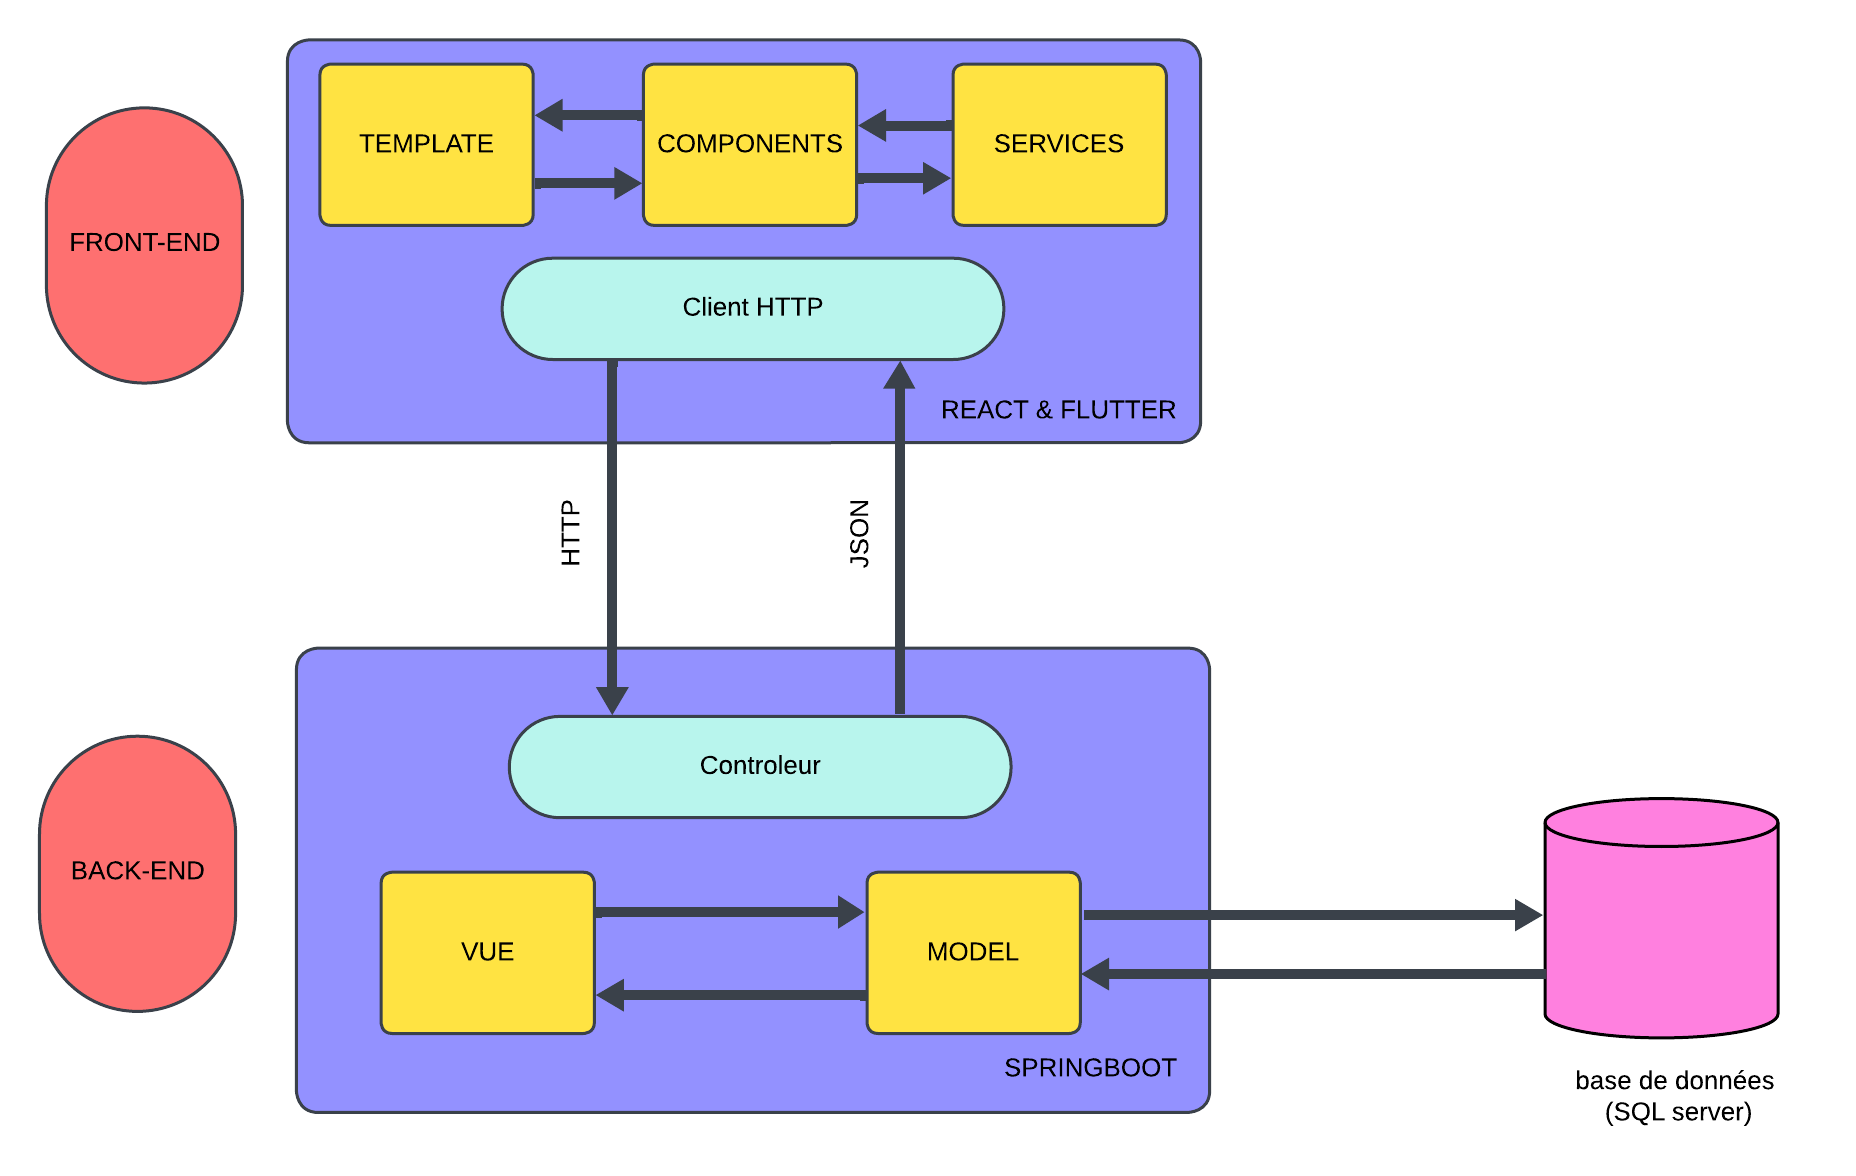
\includegraphics[height=12cm,width=15cm]{images/Brainstorming et idéation (2).png}%
    }
    \caption{Figure d'architecture du systéme}%
\end{figure}
\vspace{-1cm}
\section{Environnement de travail}

\vspace{-3mm}
Dans cette partie, nous nous intéressons d’abord à l’étude de l’environnement technique disponible pour la réalisation de mon projet. Ensuite, je justifie les choix pris en matière d’environnement logiciel pour mener à terme la partie applicative.
\vspace{-1cm}

% Partie Environnement logiciel
\section{Environnement logiciel}

\vspace{-4mm}

\subsection{Lucidchart}
\vspace{-3mm}
Lucidchart est une plateforme de collaboration en ligne, basée sur le cloud, permettant la création de diagrammes et la visualisation de données, et autres schémas conceptuels [4].
\begin{figure}[H]
    \centering
    \setlength{\fboxsep}{5pt}
    \setlength{\fboxrule}{0.5pt}
    \fbox{
\includegraphics[height=4cm,width=8cm]{images/lucidchart.png}}
    \caption{Logo Lucidchart}
\end{figure}
\vspace{-1.2cm}

\subsection{Figma}
\vspace{-3mm}
Figma est un éditeur de graphiques vectoriels et un outil de prototypage. Il est principalement basé sur le web, avec des fonctionnalités hors ligne supplémentaires activées par des applications de bureau pour macOS et Windows [5].
\begin{figure}[H]
    \centering
    \setlength{\fboxsep}{5pt}
    \setlength{\fboxrule}{0.5pt}
    \fbox{
\includegraphics[height=4cm,width=8cm]{images/figma.png}}
    \caption{Logo Figma}
\end{figure}
\vspace{-1.2cm}

% Partie Environnement de développement
\section{Environnement de développement}

\vspace{-3mm}

\subsection{Visual Studio Code}
\vspace{-3mm}
Visual Studio Code est un éditeur de code extensible développé par Microsoft pour Windows, Linux et macOS. Les fonctionnalités incluent la prise en charge du débogage, la mise en évidence de la syntaxe, la complétion intelligente du code, les snippets, la refactorisation du code et Git intégré [6]. 
\begin{figure}[H]
    \centering
    \setlength{\fboxsep}{5pt}
    \setlength{\fboxrule}{0.5pt}
    \fbox{
\includegraphics[height=4cm,width=8cm]{images/vscode.png}}
    \caption{Logo Visual Studio Code}
\end{figure}
\vspace{-1.5cm}

\subsection{IntelliJ IDEA}
\vspace{-4mm}
IntelliJ IDEA, également appelé « IntelliJ », « IDEA » ou « IDJ », est un environnement de développement destiné au développement de logiciels informatiques reposant sur la technologie Java [7]. 
\begin{figure}[H]
    \centering
    \setlength{\fboxsep}{5pt}
    \setlength{\fboxrule}{0.5pt}
    \fbox{
\includegraphics[height=4cm,width=8cm]{images/intellij.png}}
    \caption{Logo IntelliJ IDEA}
\end{figure}

\subsection{Android Studio}
\vspace{-4mm}
Android Studio est un environnement de développement pour développer des applications mobiles Android. Il est basé sur IntelliJ IDEA et utilise le moteur de production Gradle. Il peut être téléchargé sous les systèmes d'exploitation Windows, macOS, Chrome OS et Linux [8].
\begin{figure}[H]
    \centering
    \setlength{\fboxsep}{5pt}
    \setlength{\fboxrule}{0.5pt}
    \fbox{
\includegraphics[height=4cm,width=8cm]{images/androidstudio.png}}
    \caption{Logo Android Studio}
\end{figure}

% Autres outils pertinents
\subsection{Postman}
\vspace{-4mm}
Postman est une application permettant de tester des API, créée en 2012 par Abhinav Asthana, Ankit Sobti et Abhijit Kane à Bangalore pour répondre à une problématique de test d'API partageable [9].
\begin{figure}[H]
    \centering
    \setlength{\fboxsep}{5pt}
    \setlength{\fboxrule}{0.5pt}
    \fbox{
\includegraphics[height=4cm,width=8cm]{images/postman.png}}
    \caption{Logo Postman}
\end{figure}

\vspace{-2cm}
\section{Conclusion }
\vspace{-4mm}
Ce chapitre a présenté l'environnement de travail, les outils logiciels, les frameworks et les langages de programmation utilisés pour notre projet, facilitant une collaboration efficace. Nous avons défini les besoins fonctionnels et non fonctionnels, adopté la méthodologie SCRUM pour respecter les délais, et détaillé le backlog du produit ainsi que le chronogramme de travail, essentiels pour l’étude et l’analyse de notre application.

\end{sloppypar}